\documentclass[12pt, a4paper]{article}
\usepackage{../../../myconfig} % Gọi file cấu hình từ ngoài gốc vào
% ==========================================
% BẮT ĐẦU NỘI DUNG TÀI LIỆU
% ==========================================
\begin{document}

% Truyền 3 tham số: {Nhãn cam} {Chữ to chính giữa} {Chữ ở góc phải Header}
\titlebox{Chủ đề: Tích phân}{Ứng dụng tích phân trong bài toán chuyển động}{Bài toán chuyển động}

\drawdashlines{27}

% --- CÂU 1 ---
\questionShortAnswer{20}{1}{Một xe ô tô sau khi chở hết đèn đỏ đã bắt đầu chuyển động. Trong 7 phút đầu tiên vận tốc được biểu thị bằng đồ thị là đường cong parabol; biết rằng sau 5 phút thì xe đạt đến tốc độ cao nhất 900 m/phút và bắt đầu giảm tốc độ. Sau khi đi được 7 phút thì xe chuyển động đều (tham khảo hình vẽ). Quãng đường xe đi được sau 10 phút đầu tiên kể từ khi hết đèn đỏ là bao nhiêu mét?

\begin{center}
\begin{tikzpicture}[scale=0.8, >=stealth]
    % Tọa độ các điểm chính (đã scale để hình cân đối)
    % t: 0 -> 0, 5 -> 2.5, 7 -> 3.5, 10 -> 5.0
    % v: 900 -> 3.0, v(7) = 360*7 - 36*49 = 756 -> 2.52
    
    % Trục tọa độ
    \draw[->, blue!80!black, thick] (-0.5, 0) -- (6.0, 0) node[below right] {$t \text{ (phút)}$};
    \draw[->, blue!80!black, thick] (0, -0.5) -- (0, 3.8) node[right] {$v \text{ (m/phút)}$};
    
    % Gốc tọa độ O
    \node[below left] at (0,0) {$O$};
    \filldraw[fill=red!20, draw=brown!80!black] (0,0) circle (1.5pt);

    % Đường đứt nét (Dashed lines)
    \draw[dashed, blue!80!black] (0, 3) node[left, black] {$900$} -- (2.5, 3) -- (2.5, 0) node[below, black] {$5$};
    \draw[dashed, blue!80!black] (3.5, 2.52) -- (3.5, 0) node[below, black] {$7$};
    \draw[dashed, blue!80!black] (5.0, 2.52) -- (5.0, 0) node[below, black] {$10$};

    % Đồ thị
    % Parabol: v(t) = -36(t-5)^2 + 900 trong đoạn [0, 7]
    \draw[ultra thick, red!60!black, domain=0:3.5, samples=100] 
        plot (\x, {-0.48*(\x-2.5)^2 + 3.0});
        
    % Đoạn thẳng nằm ngang (chuyển động đều) từ t = 7 đến t = 10
    \draw[ultra thick, red!60!black] (3.5, 2.52) -- (5.0, 2.52);

    % Điểm mốc trên đồ thị
    \filldraw[blue!80!black] (2.5, 3) circle (1pt);
    \filldraw[blue!80!black] (3.5, 2.52) circle (1pt);
    \filldraw[blue!80!black] (5.0, 2.52) circle (1pt);
\end{tikzpicture}
\end{center}
}

% --- CÂU 2 ---
\questionShortAnswer{20}{2}{Một chất điểm chuyển động thẳng trong 19 giây với vận tốc \(v(t)\) (đơn vị: m/s) là hàm số phụ thuộc thời gian \(t\) (đơn vị: giây) có đồ thị như hình vẽ. Quãng đường chất điểm đi được từ lúc xuất phát đến khi dừng lại bằng bao nhiêu mét?

\begin{center}
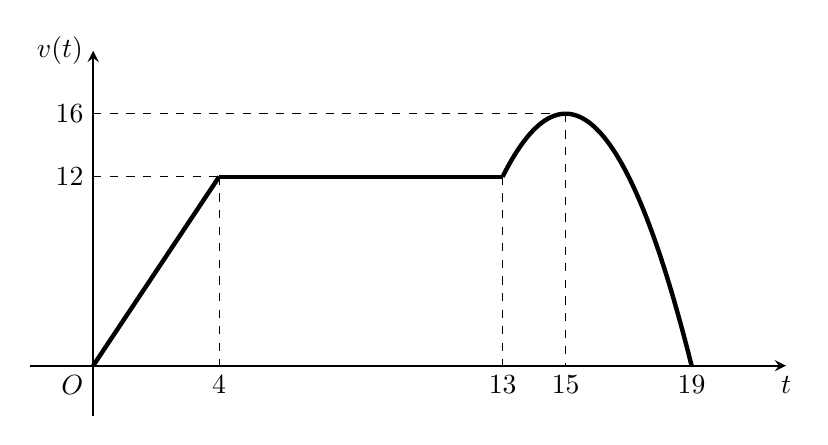
\begin{tikzpicture}[scale=0.8, >=stealth]
    % Tọa độ tỉ lệ: x = t/2, y = v/4 để hình cân đối
    % t = 0 (0,0)
    % t = 4 (2, 3) [v=12]
    % t = 13 (6.5, 3) [v=12]
    % t = 15 (7.5, 4) [v=16 - Đỉnh parabol]
    % t = 19 (9.5, 0) [v=0]

    % Trục tọa độ
    \draw[->, thick] (-1, 0) -- (11, 0) node[below] {$t$};
    \draw[->, thick] (0, -0.8) -- (0, 5) node[left] {$v(t)$};

    % Gốc tọa độ O
    \node[below left] at (0,0) {$O$};

    % Đường đứt nét (Dashed lines)
    \draw[dashed] (0, 3) node[left] {$12$} -- (6.5, 3);
    \draw[dashed] (0, 4) node[left] {$16$} -- (7.5, 4);

    \draw[dashed] (2, 3) -- (2, 0) node[below] {$4$};
    \draw[dashed] (6.5, 3) -- (6.5, 0) node[below] {$13$};
    \draw[dashed] (7.5, 4) -- (7.5, 0) node[below] {$15$};

    % Giá trị t = 19
    \node[below] at (9.5, 0) {$19$};

    % Đồ thị
    % Đoạn 1: Đoạn thẳng từ O đến (4, 12)
    \draw[ultra thick] (0, 0) -- (2, 3);

    % Đoạn 2: Đoạn thẳng nằm ngang từ t=4 đến t=13
    \draw[ultra thick] (2, 3) -- (6.5, 3);

    % Đoạn 3: Parabol đi qua (13,12), đỉnh (15,16), và cắt Oy tại (19,0)
    % Công thức: v = -t^2 + 30t - 209 => v = -(t-15)^2 + 16
    \draw[ultra thick, domain=6.5:9.5, samples=100] 
        plot (\x, {-(\x*2-15)^2/4 + 4});

\end{tikzpicture}
\end{center}
}

% --- CÂU 3 ---
\questionShortAnswer{28}{3}{Để đảm bảo an toàn khi lưu thông trên đường, các xe ô tô khi dừng đèn đỏ phải cách nhau tối thiểu 1m. Một ô tô A đang chạy với vận tốc 12m/s bỗng gặp ô tô B đang dừng đèn đỏ nên ô tô A hãm phanh và chuyển động chậm dần đều với vận tốc được biểu thị bởi công thức \(v_A(t) = 12 - 3t\) (m/s). Hỏi để hai ô tô đạt khoảng cách an toàn khi dừng lại thì ô tô A phải hãm phanh khi cách ô tô B một khoảng ít nhất là bao nhiêu mét?
}


% --- CÂU 4 ---
\questionShortAnswer{28}{4}{Một ô tô bắt đầu chuyển động nhanh dần đều với vận tốc \(v_1(t) = 2t\) (m/s). Đi được 12 giây, người lái xe gặp chướng ngại vật và phanh gấp, ô tô tiếp tục chuyển động chậm dần đều với gia tốc \(a = -12\) (m/s\(^2\)). Tính quãng đường \(s\) (m) đi được của ô tô từ lúc bắt đầu chuyển động đến khi dừng hẳn?
}

% --- CÂU 5 ---
\questionShortAnswer{28}{5}{Một xe chuyển động với vận tốc thay đổi theo thời gian là \(v(t) = 3at^2 + bt\). Gọi \(S(t)\) là quãng đường đi được sau \(t\) giây. Biết rằng sau 4 giây thì quãng đường đi được là 144 m, và sau 6 giây thì quãng đường đi được là 468 m. Tính quãng đường xe đi được sau 10 giây.
}

% --- CÂU 6 ---
\questionShortAnswer{28}{6}{Một chất điểm \(A\) xuất phát từ \(O\), chuyển động thẳng với vận tốc biến thiên theo thời gian bởi quy luật \(v(t) = \dfrac{2}{100}t^2 + \dfrac{17}{30}t\) (m/s) trong đó \(t\) (giây) là khoảng thời gian tính từ lúc \(A\) bắt đầu chuyển động. Từ trạng thái nghỉ, một chất điểm \(B\) cũng xuất phát từ \(O\), chuyển động thẳng cùng hướng với \(A\) nhưng chậm hơn 10 giây so với \(A\) và có gia tốc bằng \(a\) (m/s\(^2\)) (\(a\) là hằng số). Sau khi \(B\) xuất phát được 15 giây thì đuổi kịp \(A\). Vận tốc của \(B\) tại thời điểm đuổi kịp \(A\) bằng bao nhiêu?
}

% --- CÂU 7 ---
\questionShortAnswer{20}{7}{Trong một trò chơi điện tử, có bốn chất điểm \(A, B, C, D\) đang di chuyển trên các đường thẳng song song như hình vẽ. Lập trình viên đã thiết lập vận tốc của các chất điểm \(A, B, C\) lần lượt là: \(v_A(t) = t + 2\), \(v_B(t) = 2t\), \(v_C(t) = 11 - 2t\).

(Trong đó \(t\) tính bằng giây từ lúc bắt đầu chuyển động, \(v\) tính bằng m/s. Giả thiết rằng khi \(v < 0\) thì chất điểm di chuyển từ phải qua trái).

Biết vận tốc của chất điểm \(D\) tại mỗi thời điểm bất kỳ được tính bằng vận tốc nhỏ nhất của ba chất điểm \(A, B, C\). Hỏi quãng đường chất điểm \(D\) đi được trong 5 giây đầu tiên bằng bao nhiêu mét?

\begin{center}
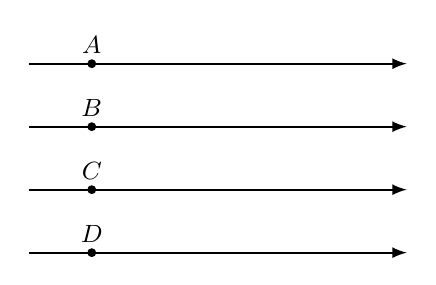
\begin{tikzpicture}[>=latex, scale=0.8]
    % Vẽ các đường thẳng song song
    \draw[thick, ->] (0, 3) -- (6, 3);
    \draw[thick, ->] (0, 2) -- (6, 2);
    \draw[thick, ->] (0, 1) -- (6, 1);
    \draw[thick, ->] (0, 0) -- (6, 0);
    
    % Đánh dấu các điểm
    \fill (1, 3) circle (2pt);
    \node[above] at (1, 3) {\small $A$};
    \fill (1, 2) circle (2pt);
    \node[above] at (1, 2) {\small $B$};
    \fill (1, 1) circle (2pt);
    \node[above] at (1, 1) {\small $C$};
    \fill (1, 0) circle (2pt);
    \node[above] at (1, 0) {\small $D$};
\end{tikzpicture}
\end{center}
}

% --- CÂU 8 ---
\questionShortAnswer{28}{8}{Người ta thả một vật từ một vị trí trên cao cho rơi xuống mặt đất theo phương thẳng đứng. Biết gia tốc trọng trường tại nơi thả vật bằng \(9,8\) m/s\(^2\). Giả sử lực tác động của không khí đối với vật trong quá trình rơi là không đáng kể. Biết rằng sau 4 giây thì vật bắt đầu chạm mặt đất. Hỏi vị trí của vật trước khi thả rơi cao bao nhiêu mét so với mặt đất? (kết quả làm tròn đến hàng phần mười)
}

% --- CÂU 9 ---
\questionShortAnswer{28}{9}{Một viên đạn được bắn thẳng đứng lên trên từ độ cao 2 m với vận tốc tại thời điểm \(t\) cho bởi công thức \(v(t) = 100 - 9,8t\) (m/s), (\(t = 0\) là thời điểm viên đạn được bắn lên). Tìm độ cao (tính theo km) của viên đạn so với mặt đất ở thời điểm 1 giây sau khi viên đạn đạt độ cao lớn nhất (làm tròn đến hàng phần trăm).
}

% --- CÂU 10 ---
\questionShortAnswer{25}{10}{Người ta cho một chiếc xe điện mô hình chạy thử nghiệm trên một đường thẳng trong 24 giây với vận tốc
\[
v(t) = \begin{cases}
\dfrac{1}{2}t & \text{khi } 0 \leq t \leq 8 \\
4 & \text{khi } 8 < t < 16 \\
-\dfrac{1}{2}t + 12 & \text{khi } 16 \leq t \leq 24
\end{cases}
\]
(decimet/giây), trong đó \(t\) là khoảng thời gian tính bằng giây kể từ lúc xe bắt đầu chuyển động. Trong 24 giây chạy thử nghiệm đó, chiếc xe mô hình đi được quãng đường bao nhiêu decimet?
}




\end{document}